\documentclass[]{article}
\usepackage{lmodern}
\usepackage{amssymb,amsmath}
\usepackage{ifxetex,ifluatex}
\usepackage{fixltx2e} % provides \textsubscript
\ifnum 0\ifxetex 1\fi\ifluatex 1\fi=0 % if pdftex
  \usepackage[T1]{fontenc}
  \usepackage[utf8]{inputenc}
\else % if luatex or xelatex
  \ifxetex
    \usepackage{mathspec}
  \else
    \usepackage{fontspec}
  \fi
  \defaultfontfeatures{Ligatures=TeX,Scale=MatchLowercase}
\fi
% use upquote if available, for straight quotes in verbatim environments
\IfFileExists{upquote.sty}{\usepackage{upquote}}{}
% use microtype if available
\IfFileExists{microtype.sty}{%
\usepackage{microtype}
\UseMicrotypeSet[protrusion]{basicmath} % disable protrusion for tt fonts
}{}
\usepackage[margin=1in]{geometry}
\usepackage{hyperref}
\hypersetup{unicode=true,
            pdftitle={Normal\_cor\_simulation},
            pdfauthor={Xuelong Wang},
            pdfborder={0 0 0},
            breaklinks=true}
\urlstyle{same}  % don't use monospace font for urls
\usepackage{graphicx,grffile}
\makeatletter
\def\maxwidth{\ifdim\Gin@nat@width>\linewidth\linewidth\else\Gin@nat@width\fi}
\def\maxheight{\ifdim\Gin@nat@height>\textheight\textheight\else\Gin@nat@height\fi}
\makeatother
% Scale images if necessary, so that they will not overflow the page
% margins by default, and it is still possible to overwrite the defaults
% using explicit options in \includegraphics[width, height, ...]{}
\setkeys{Gin}{width=\maxwidth,height=\maxheight,keepaspectratio}
\IfFileExists{parskip.sty}{%
\usepackage{parskip}
}{% else
\setlength{\parindent}{0pt}
\setlength{\parskip}{6pt plus 2pt minus 1pt}
}
\setlength{\emergencystretch}{3em}  % prevent overfull lines
\providecommand{\tightlist}{%
  \setlength{\itemsep}{0pt}\setlength{\parskip}{0pt}}
\setcounter{secnumdepth}{5}
% Redefines (sub)paragraphs to behave more like sections
\ifx\paragraph\undefined\else
\let\oldparagraph\paragraph
\renewcommand{\paragraph}[1]{\oldparagraph{#1}\mbox{}}
\fi
\ifx\subparagraph\undefined\else
\let\oldsubparagraph\subparagraph
\renewcommand{\subparagraph}[1]{\oldsubparagraph{#1}\mbox{}}
\fi

%%% Use protect on footnotes to avoid problems with footnotes in titles
\let\rmarkdownfootnote\footnote%
\def\footnote{\protect\rmarkdownfootnote}

%%% Change title format to be more compact
\usepackage{titling}

% Create subtitle command for use in maketitle
\newcommand{\subtitle}[1]{
  \posttitle{
    \begin{center}\large#1\end{center}
    }
}

\setlength{\droptitle}{-2em}

  \title{Normal\_cor\_simulation}
    \pretitle{\vspace{\droptitle}\centering\huge}
  \posttitle{\par}
    \author{Xuelong Wang}
    \preauthor{\centering\large\emph}
  \postauthor{\par}
      \predate{\centering\large\emph}
  \postdate{\par}
    \date{2018-07-22}

\usepackage{booktabs}
\usepackage{longtable}
\usepackage{array}
\usepackage{multirow}
\usepackage[table]{xcolor}
\usepackage{wrapfig}
\usepackage{float}
\usepackage{colortbl}
\usepackage{pdflscape}
\usepackage{tabu}
\usepackage{threeparttable}
\usepackage{threeparttablex}
\usepackage[normalem]{ulem}
\usepackage{makecell}

\usepackage{float,amsmath, bbm, siunitx, bm}
\floatplacement{figure}{H}
\newcommand{\indep}{\rotatebox[origin=c]{90}{$\models$}}

\begin{document}
\maketitle

{
\setcounter{tocdepth}{2}
\tableofcontents
}
\section{Motivation}\label{motivation}

\section{Simulation result}\label{simulation-result}

\subsection{Setup}\label{setup}

\subsubsection{Averaged estimation}\label{averaged-estimation}

\rowcolors{2}{gray!80}{white}

\begin{table}[!h]

\caption{\label{tab:full data}correlation-0.1-rank}
\centering
\begin{tabular}[t]{r|r|r|r|r|r}
\hiderowcolors
\hline
\multicolumn{3}{c|}{Main} & \multicolumn{3}{|c}{Interaction} \\
\cline{1-3} \cline{4-6}
true\_main & GCTA\_main & prop\_main & true\_interaction & GCTA\_interaction & prop\_interaction\\
\hline
\showrowcolors
3.273011 & 3.2917501 & 3.5821454 & 6.269756 & 8.9266748 & 6.3453264\\
\hline
0.000000 & 0.5443885 & 0.5044931 & 0.000000 & 1.9384712 & 0.9316854\\
\hline
3.796410 & 3.1264892 & 3.7124981 & 4.785749 & 3.1161925 & 4.7414871\\
\hline
0.000000 & 0.5343199 & 0.5359537 & 0.000000 & 0.7696360 & 0.9454778\\
\hline
2.562346 & 1.7143087 & 2.3482984 & 5.601250 & 4.2969854 & 5.6991445\\
\hline
0.000000 & 0.3453015 & 0.4253327 & 0.000000 & 0.9588671 & 1.0082503\\
\hline
\end{tabular}
\end{table}

\rowcolors{2}{white}{white} \rowcolors{2}{gray!80}{white}

\begin{table}[!h]

\caption{\label{tab:full data}correlation-0.2-rank}
\centering
\begin{tabular}[t]{r|r|r|r|r|r}
\hiderowcolors
\hline
\multicolumn{3}{c|}{Main} & \multicolumn{3}{|c}{Interaction} \\
\cline{1-3} \cline{4-6}
true\_main & GCTA\_main & prop\_main & true\_interaction & GCTA\_interaction & prop\_interaction\\
\hline
\showrowcolors
3.287854 & 2.5921070 & 3.1436565 & 6.770908 & 11.2012351 & 6.7164432\\
\hline
0.000000 & 0.6156821 & 0.5132497 & 0.000000 & 2.3052595 & 1.0607838\\
\hline
3.451079 & 1.9155244 & 3.1663861 & 4.501921 & 1.6658913 & 4.4551279\\
\hline
0.000000 & 0.4702985 & 0.4613175 & 0.000000 & 0.4234275 & 0.9870434\\
\hline
2.277031 & 1.1033043 & 1.9360422 & 4.852822 & 1.4949975 & 4.2776881\\
\hline
0.000000 & 0.3723105 & 0.3711155 & 0.000000 & 0.4598318 & 0.9419064\\
\hline
\end{tabular}
\end{table}

\rowcolors{2}{white}{white} \rowcolors{2}{gray!80}{white}

\begin{table}[!h]

\caption{\label{tab:full data}correlation-0.3-rank}
\centering
\begin{tabular}[t]{r|r|r|r|r|r}
\hiderowcolors
\hline
\multicolumn{3}{c|}{Main} & \multicolumn{3}{|c}{Interaction} \\
\cline{1-3} \cline{4-6}
true\_main & GCTA\_main & prop\_main & true\_interaction & GCTA\_interaction & prop\_interaction\\
\hline
\showrowcolors
3.191655 & 2.0751094 & 3.1778233 & 7.531216 & 12.0263149 & 7.1408985\\
\hline
0.000000 & 0.5307726 & 0.5135604 & 0.000000 & 1.9506731 & 1.1291242\\
\hline
3.339649 & 1.7675255 & 3.3043715 & 4.050892 & 0.5155483 & 3.5605773\\
\hline
0.000000 & 0.4893117 & 0.4962328 & 0.000000 & 0.2001673 & 0.8826682\\
\hline
2.038114 & 0.9754073 & 2.0122458 & 4.783040 & 0.8566086 & 4.5923752\\
\hline
0.000000 & 0.4133394 & 0.4072330 & 0.000000 & 0.2153063 & 0.8332746\\
\hline
\end{tabular}
\end{table}

\rowcolors{2}{white}{white} \rowcolors{2}{gray!80}{white}

\begin{table}[!h]

\caption{\label{tab:full data}correlation-0.4-rank}
\centering
\begin{tabular}[t]{r|r|r|r|r|r}
\hiderowcolors
\hline
\multicolumn{3}{c|}{Main} & \multicolumn{3}{|c}{Interaction} \\
\cline{1-3} \cline{4-6}
true\_main & GCTA\_main & prop\_main & true\_interaction & GCTA\_interaction & prop\_interaction\\
\hline
\showrowcolors
3.083154 & 2.3328907 & 3.1190410 & 7.894065 & 12.7649792 & 7.1558509\\
\hline
0.000000 & 0.5965657 & 0.5654936 & 0.000000 & 1.7175563 & 0.9890324\\
\hline
3.151569 & 1.9214769 & 3.2288690 & 3.468205 & 0.4418272 & 2.5874831\\
\hline
0.000000 & 0.4450802 & 0.4358622 & 0.000000 & 0.1617832 & 0.7005672\\
\hline
1.774852 & 0.5980890 & 1.5768253 & 3.977908 & 0.5104431 & 2.7801760\\
\hline
0.000000 & 0.2518925 & 0.3319370 & 0.000000 & 0.2231496 & 0.7683978\\
\hline
\end{tabular}
\end{table}

\rowcolors{2}{white}{white} \rowcolors{2}{gray!80}{white}

\begin{table}[!h]

\caption{\label{tab:full data}correlation-0.5-rank}
\centering
\begin{tabular}[t]{r|r|r|r|r|r}
\hiderowcolors
\hline
\multicolumn{3}{c|}{Main} & \multicolumn{3}{|c}{Interaction} \\
\cline{1-3} \cline{4-6}
true\_main & GCTA\_main & prop\_main & true\_interaction & GCTA\_interaction & prop\_interaction\\
\hline
\showrowcolors
2.893748 & 2.3024869 & 2.4028098 & 7.691212 & 10.7845926 & 6.5634685\\
\hline
0.000000 & 0.4784659 & 0.4045158 & 0.000000 & 1.4360667 & 1.0715056\\
\hline
2.871685 & 1.3541603 & 2.4856693 & 2.945046 & 0.1016010 & 1.8439252\\
\hline
0.000000 & 0.4032703 & 0.4648654 & 0.000000 & 0.0768577 & 0.7091286\\
\hline
1.614075 & 0.4694316 & 1.3682154 & 3.056443 & 0.3351225 & 2.1218839\\
\hline
0.000000 & 0.2108956 & 0.2900643 & 0.000000 & 0.2204598 & 0.7663524\\
\hline
\end{tabular}
\end{table}

\rowcolors{2}{white}{white} \rowcolors{2}{gray!80}{white}

\begin{table}[!h]

\caption{\label{tab:full data}correlation-0.6-rank}
\centering
\begin{tabular}[t]{r|r|r|r|r|r}
\hiderowcolors
\hline
\multicolumn{3}{c|}{Main} & \multicolumn{3}{|c}{Interaction} \\
\cline{1-3} \cline{4-6}
true\_main & GCTA\_main & prop\_main & true\_interaction & GCTA\_interaction & prop\_interaction\\
\hline
\showrowcolors
2.862072 & 2.4174144 & 2.6436607 & 8.039859 & 11.0860764 & 8.6552185\\
\hline
0.000000 & 0.5401346 & 0.5119302 & 0.000000 & 1.2308141 & 1.1244137\\
\hline
2.599112 & 1.6483702 & 2.8042186 & 2.438889 & 0.1140950 & 1.5863575\\
\hline
0.000000 & 0.4224303 & 0.3902903 & 0.000000 & 0.1066162 & 0.6650055\\
\hline
1.373710 & 0.3102861 & 1.3018094 & 2.707392 & 0.1738568 & 1.8306026\\
\hline
0.000000 & 0.1687992 & 0.3355386 & 0.000000 & 0.1347137 & 0.6639718\\
\hline
\end{tabular}
\end{table}

\rowcolors{2}{white}{white} \rowcolors{2}{gray!80}{white}

\begin{table}[!h]

\caption{\label{tab:full data}correlation-0.7-rank}
\centering
\begin{tabular}[t]{r|r|r|r|r|r}
\hiderowcolors
\hline
\multicolumn{3}{c|}{Main} & \multicolumn{3}{|c}{Interaction} \\
\cline{1-3} \cline{4-6}
true\_main & GCTA\_main & prop\_main & true\_interaction & GCTA\_interaction & prop\_interaction\\
\hline
\showrowcolors
2.762765 & 2.5981790 & 2.5301655 & 8.381747 & 11.9652031 & 10.7651609\\
\hline
0.000000 & 0.5237298 & 0.4600912 & 0.000000 & 1.2560767 & 1.3741490\\
\hline
2.203353 & 1.3538424 & 2.2054306 & 1.692767 & 0.0442788 & 0.6312460\\
\hline
0.000000 & 0.3606873 & 0.4077517 & 0.000000 & 0.0651771 & 0.5678627\\
\hline
1.151067 & 0.4668372 & 1.0171875 & 1.811800 & 0.1635264 & 0.9408967\\
\hline
0.000000 & 0.1932195 & 0.2996236 & 0.000000 & 0.1631234 & 0.5278105\\
\hline
\end{tabular}
\end{table}

\rowcolors{2}{white}{white} \rowcolors{2}{gray!80}{white}

\begin{table}[!h]

\caption{\label{tab:full data}correlation-0.8-rank}
\centering
\begin{tabular}[t]{r|r|r|r|r|r}
\hiderowcolors
\hline
\multicolumn{3}{c|}{Main} & \multicolumn{3}{|c}{Interaction} \\
\cline{1-3} \cline{4-6}
true\_main & GCTA\_main & prop\_main & true\_interaction & GCTA\_interaction & prop\_interaction\\
\hline
\showrowcolors
2.6938022 & 2.6075374 & 2.4276241 & 8.548136 & 11.5919954 & 12.3174931\\
\hline
0.0000000 & 0.4111341 & 0.4786533 & 0.000000 & 1.1345748 & 1.4616026\\
\hline
1.9258045 & 1.3098241 & 1.9241811 & 1.128533 & 0.0541264 & 0.0042766\\
\hline
0.0000000 & 0.3305982 & 0.3399465 & 0.000000 & 0.0762302 & 0.4628433\\
\hline
0.8749072 & 0.4420723 & 0.9004700 & 1.302277 & 0.0870159 & 0.4794344\\
\hline
0.0000000 & 0.1892886 & 0.2690165 & 0.000000 & 0.0929880 & 0.4242552\\
\hline
\end{tabular}
\end{table}

\rowcolors{2}{white}{white} \rowcolors{2}{gray!80}{white}

\begin{table}[!h]

\caption{\label{tab:full data}correlation-0.9-rank}
\centering
\begin{tabular}[t]{r|r|r|r|r|r}
\hiderowcolors
\hline
\multicolumn{3}{c|}{Main} & \multicolumn{3}{|c}{Interaction} \\
\cline{1-3} \cline{4-6}
true\_main & GCTA\_main & prop\_main & true\_interaction & GCTA\_interaction & prop\_interaction\\
\hline
\showrowcolors
2.6124061 & 2.7289938 & 2.2996102 & 8.8643704 & 11.8996553 & 16.6313905\\
\hline
0.0000000 & 0.5120883 & 0.5066546 & 0.0000000 & 0.9770764 & 1.7281144\\
\hline
1.6765453 & 1.3756480 & 1.7078619 & 0.5539569 & 0.0316277 & -0.1769137\\
\hline
0.0000000 & 0.3294642 & 0.3581214 & 0.0000000 & 0.0546656 & 0.4286480\\
\hline
0.6315223 & 0.3686161 & 0.6189097 & 0.6257508 & 0.0816362 & 0.1575732\\
\hline
0.0000000 & 0.1721345 & 0.2338492 & 0.0000000 & 0.0822467 & 0.4140326\\
\hline
\end{tabular}
\end{table}

\rowcolors{2}{white}{white}

\clearpage

\subsubsection{Histgram of 100
iterations}\label{histgram-of-100-iterations}

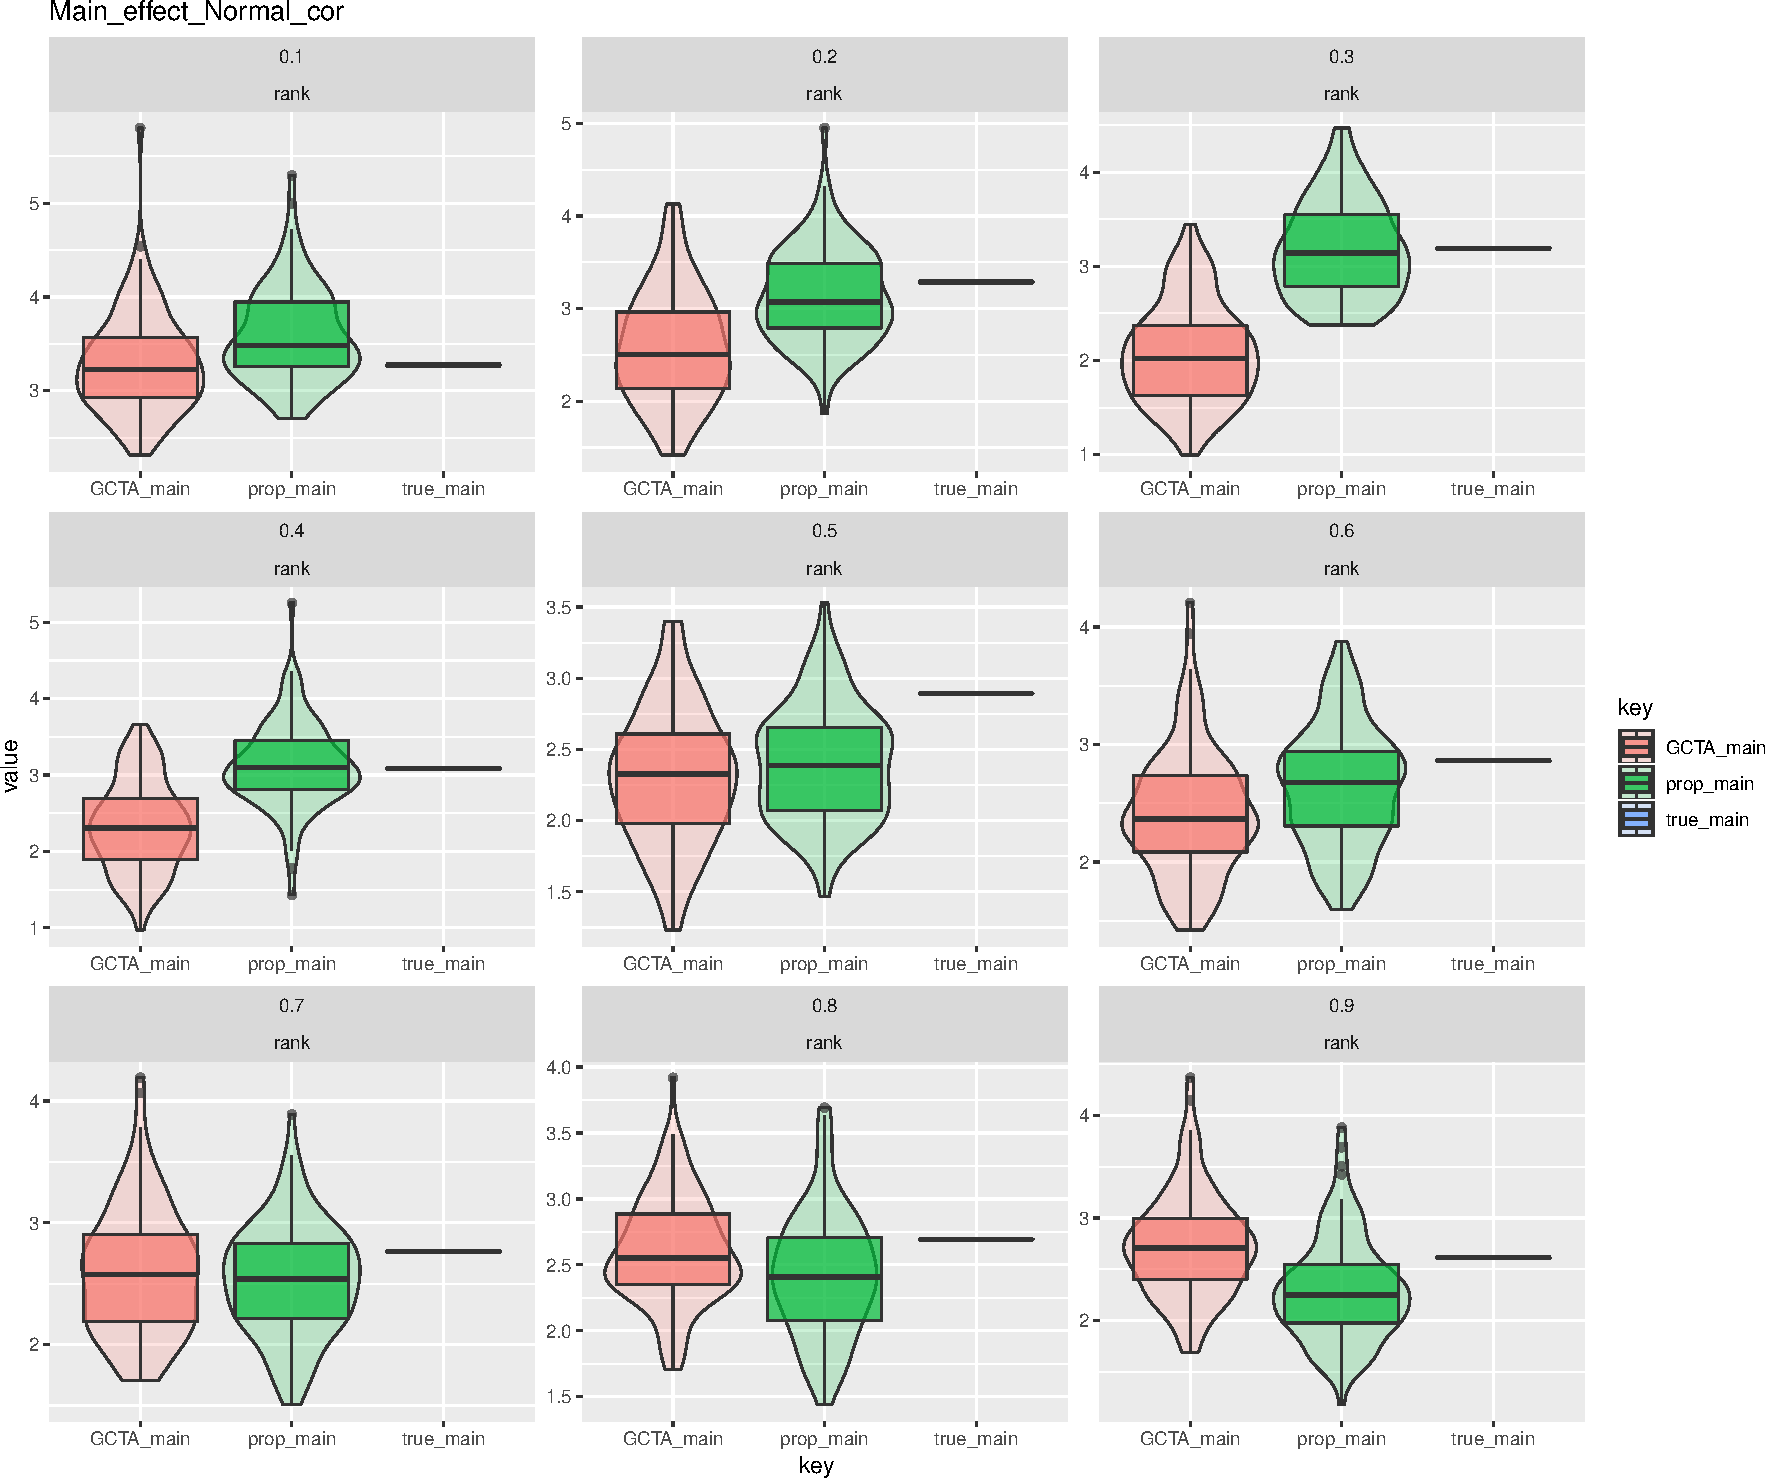
\includegraphics{Norl_cor_simulation_files/figure-latex/normal_main-1.pdf}

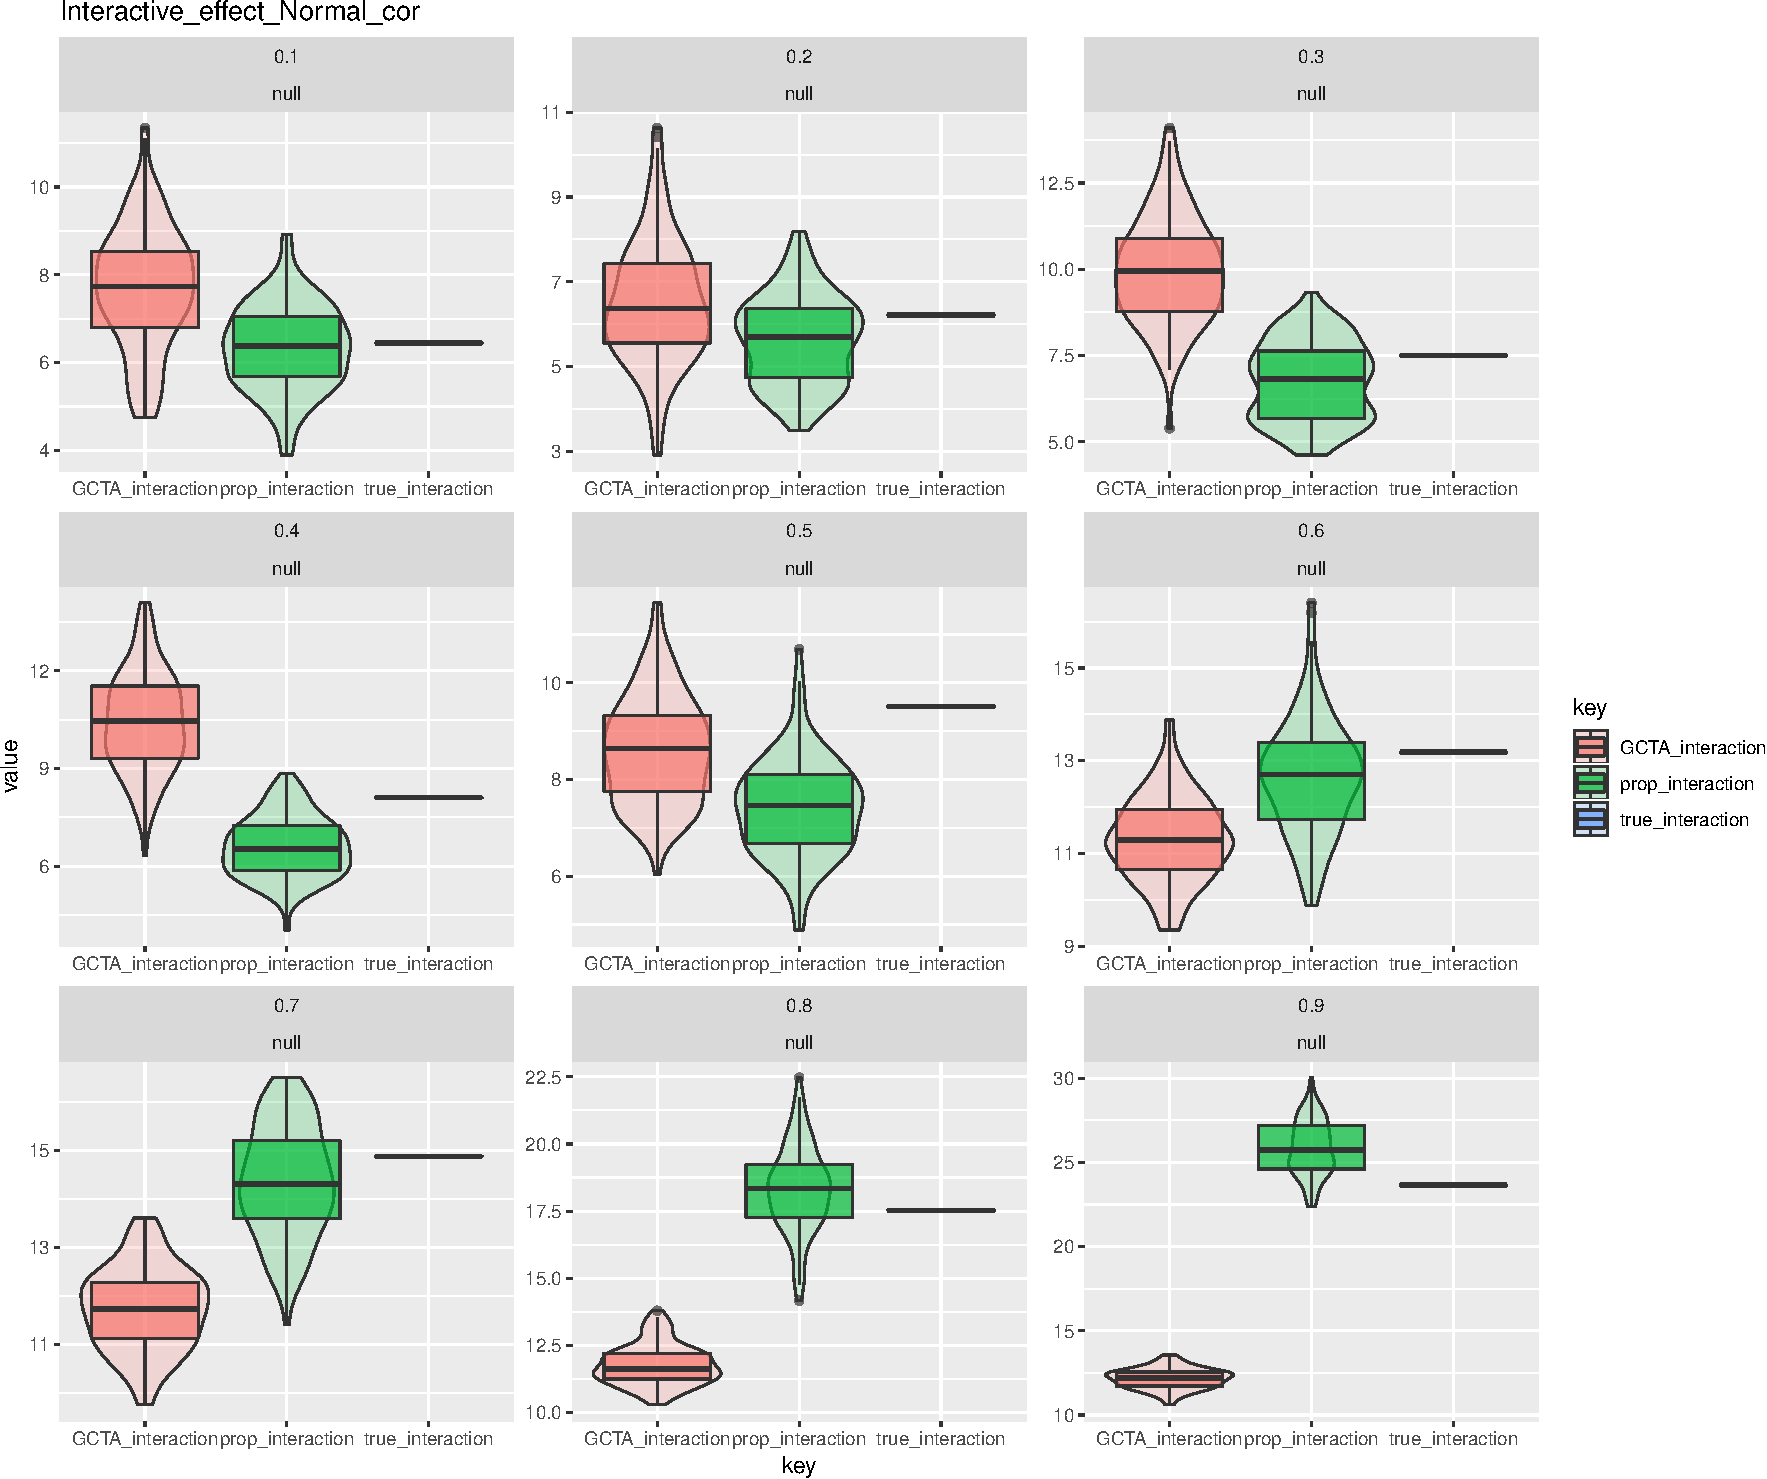
\includegraphics{Norl_cor_simulation_files/figure-latex/normal_inter-1.pdf}

\section{Conclusion}\label{conclusion}

\section{Further work}\label{further-work}


\end{document}
